\documentclass[conference]{IEEEtran}
\IEEEoverridecommandlockouts
% The preceding line is only needed to identify funding in the first footnote. If that is unneeded, please comment it out.
\usepackage{cite}
\usepackage{amsmath,amssymb,amsfonts}
\usepackage{algorithmic}
\usepackage{graphicx}
\usepackage{textcomp}
\usepackage{xcolor}
\usepackage{tabularx}
\usepackage{array}
\def\BibTeX{{\rm B\kern-.05em{\sc i\kern-.025em b}\kern-.08em
    T\kern-.1667em\lower.7ex\hbox{E}\kern-.125emX}}
\renewcommand{\abstractname}{\textmd{Abstract}}
\begin{document}

\title{A Comparative Review of Convolutional Neural Networks and Vision Transformers for Image Classification\\

\thanks
}
\author{
\IEEEauthorblockN{1\textsuperscript{st} Rajneesh Tiwari}
\IEEEauthorblockA{\textit{Noida Institute of Engineering and Technology (NIET)}\\
Greater Noida, India\\
0241csds335@niet.co.in}
\and
\IEEEauthorblockN{2\textsuperscript{nd} Priyanshu Aswal}
\IEEEauthorblockA{\textit{Noida Institute of Engineering and Technology (NIET)}\\
Greater Noida, India}
\and
\IEEEauthorblockN{3\textsuperscript{rd} Pratham Sehrawat}
\IEEEauthorblockA{\textit{Noida Institute of Engineering and Technology (NIET)}\\
Greater Noida, India}
}
\maketitle

\begin{abstract}
\normalfont
Convolutional Neural Networks (CNNs) have been widely used for image classification because of their ability to learn spatial features through convolutional operations. In recent years, Vision Transformers (ViTs) have emerged as an alternative architecture that applies self-attention mechanisms to capture global relationships within images. This paper presents a comparative review of CNNs and Vision Transformers for image classification. It discusses their fundamental architectures, feature extraction mechanisms, computational requirements, strengths, limitations, and applications. The review also examines how the two approaches differ in their ability to model local and global visual information. Based on the reviewed literature, the paper highlights the factors that influence the selection of CNNs or Vision Transformers for different image classification tasks and discusses the potential direction of future research in this area.

\end{abstract}

\begin{IEEEkeywords}
\textit{Convolutional Neural Networks, Vision Transformers, Image Classification, Deep Learning, Computer Vision, Self-Attention}
\end{IEEEkeywords}

\section{Introduction}

Image classification is one of the fundamental tasks in computer vision, with applications in areas such as medical imaging, autonomous systems, security, agriculture, and industrial inspection. The objective of image classification is to assign an input image to one or more predefined categories based on its visual characteristics. The rapid development of deep learning has significantly improved the performance of image classification systems by enabling models to automatically learn useful features directly from image data.

Convolutional Neural Networks (CNNs) have been one of the most widely used deep learning architectures for image classification. CNNs use convolutional operations to extract spatial and hierarchical features from images. Their ability to learn local patterns such as edges, textures, and shapes has made them highly effective for a wide range of computer vision tasks. Over time, several CNN architectures have been developed with improvements in depth, feature extraction, computational efficiency, and classification accuracy.

More recently, Vision Transformers (ViTs) have emerged as an alternative approach to conventional convolution-based architectures. Inspired by the Transformer architecture originally developed for natural language processing, Vision Transformers divide an image into smaller patches and process these patches using self-attention mechanisms. Unlike CNNs, which primarily focus on local spatial relationships through convolutional operations, Vision Transformers can model relationships between different regions of an image using global attention. This has created a new direction for research in image classification and other computer vision applications.

Although both CNNs and Vision Transformers have demonstrated strong performance, they differ considerably in their architectural design, feature extraction mechanisms, computational requirements, data requirements, and ability to capture visual information. Understanding these differences is important when selecting an appropriate architecture for a particular image classification problem.

This paper presents a comparative review of CNNs and Vision Transformers for image classification. It discusses the fundamental principles and architectures of both approaches, their feature extraction mechanisms, computational characteristics, strengths, limitations, and practical applications. The paper further compares their ability to capture local and global visual information and examines the factors that influence the selection of CNN-based or Transformer-based models for different image classification tasks. Finally, the review discusses current challenges and potential future research directions in this field.

\begin{figure*}[!t]
\centering
\begin{minipage}[t]{0.485\textwidth}
\centering
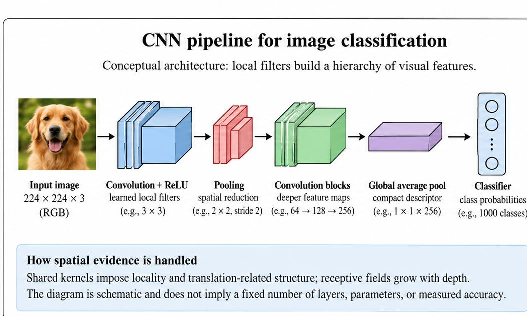
\includegraphics[width=\linewidth]{figures/cnn_architecture.pdf}
\caption{Conceptual CNN classification pipeline. The figure depicts an architecture pattern, not a measured model or performance result.}
\label{fig:cnn_pipeline}
\end{minipage}\hfill
\begin{minipage}[t]{0.485\textwidth}
\centering
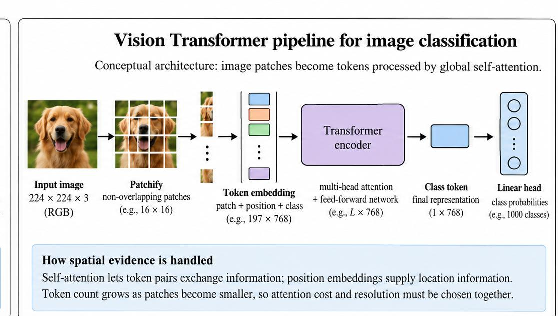
\includegraphics[width=\linewidth]{figures/vit_architecture.pdf}
\caption{Conceptual Vision Transformer classification pipeline. Patch size, token count, encoder depth, and embedding width are design choices with resource consequences.}
\label{fig:vit_pipeline}
\end{minipage}
\end{figure*}

\section{CNN Fundamentals}
Convolutional Neural Networks (CNNs) are among the most widely used deep learning architectures for image classification and computer vision tasks. Their main advantage is the ability to automatically learn hierarchical visual features directly from raw image data. Unlike traditional image-processing methods that require manually designed features, CNNs learn useful representations during the training process.

\subsection{Basic Architecture}

A typical CNN consists of convolutional layers, activation functions, pooling layers, and fully connected layers. The convolutional layers extract spatial features from an input image, while pooling layers reduce the spatial dimensions of the feature maps. The extracted features are then processed by fully connected layers to produce the final classification output.


\subsection{Convolution Operation}

The convolution operation applies a set of learnable filters, also called kernels, to the input image. Each filter moves across the image and performs element-wise multiplication followed by summation. This operation produces a feature map that represents specific visual patterns such as edges, textures, and shapes.

As the network becomes deeper, successive convolutional layers can learn increasingly complex features. Early layers generally detect simple patterns, whereas deeper layers can represent more abstract structures relevant to object recognition and image classification.

\subsection{Activation and Pooling}

CNNs commonly use nonlinear activation functions after convolution operations. The Rectified Linear Unit (ReLU) is widely used because it introduces nonlinearity while maintaining computational simplicity. Pooling operations are used to reduce the spatial dimensions of feature maps and decrease the number of parameters in subsequent layers.

Max pooling selects the maximum value within a local region, allowing the network to retain strong feature responses while reducing the spatial resolution. This can also provide a degree of robustness to small changes in the position of visual features.

\subsection{Feature Hierarchy and Classification}

The hierarchical structure of CNNs enables the network to learn representations at different levels of abstraction. Lower-level layers can capture edges and simple textures, intermediate layers can identify combinations of shapes, and deeper layers can learn high-level semantic representations.

After feature extraction, the learned representation is used for classification. Modern CNN architectures may use fully connected layers or global pooling followed by a classification layer. The final layer typically produces probabilities for the target image classes.

\subsection{CNN Architectures}

Several CNN architectures have significantly influenced the development of image classification. AlexNet demonstrated the effectiveness of deep CNNs on large-scale image recognition tasks. Later architectures such as VGG, GoogLeNet, and ResNet introduced deeper networks and architectural improvements that enhanced feature extraction and classification performance. DenseNet, MobileNetV2, and EfficientNet further explored feature reuse, mobile efficiency, and systematic model scaling \cite{krizhevsky2012,simonyan2015,szegedy2015,he2016,huang2017,sandler2018,tan2019}.

Residual Networks (ResNets), in particular, introduced residual connections that help information and gradients propagate through very deep networks. These developments have made CNNs an important foundation for modern computer vision systems.

\section{Vision Transformer Fundamentals}

Vision Transformers (ViTs) apply the Transformer architecture to image classification by representing an image as a sequence of smaller image patches. The original Transformer introduced attention-based sequence processing, while ViT adapted this design to image patches; later variants such as DeiT, Swin Transformer, Pyramid Vision Transformer, and CvT explored data efficiency, hierarchy, and convolutional tokenization \cite{vaswani2017,dosovitskiy2021,touvron2021,liu2021swin,wang2021pvt,wu2021cvt}. Unlike conventional CNNs, which primarily rely on local convolutional operations, ViTs use self-attention mechanisms to model relationships between different regions of an image.

\subsection{Patch Embedding}

In a Vision Transformer, the input image is divided into a fixed number of non-overlapping patches. Each patch is flattened into a vector and projected into a lower-dimensional embedding space. These patch embeddings form a sequence that can be processed by the Transformer encoder.

This representation allows the model to treat an image as a sequence of visual tokens. The patch size and embedding dimension influence both the computational requirements and the amount of visual information represented by each token.

\subsection{Positional Encoding}

Since the Transformer does not inherently contain information about the spatial arrangement of tokens, positional information is added to the patch embeddings. Positional embeddings allow the model to distinguish between patches based on their location within the original image.

The combination of patch embeddings and positional information provides the Transformer with both visual content and spatial context.

\subsection{Self-Attention Mechanism}

Self-attention is a central component of the Vision Transformer. It enables each image patch to interact with other patches in the sequence and learn relationships between distant regions of an image.

The attention mechanism uses query, key, and value representations to determine the importance of different tokens. This allows the model to capture global dependencies that may be difficult to represent using only local convolutional operations.

\subsection{Transformer Encoder}

The Transformer encoder consists of multiple layers containing multi-head self-attention and feed-forward neural networks. Layer normalization and residual connections are used to improve the stability and effectiveness of deep Transformer models.

By stacking multiple encoder layers, the network can progressively learn more complex relationships among image patches.

\subsection{Classification}

For image classification, a special classification token can be added to the sequence of image patches. After processing the sequence through the Transformer encoder, the representation associated with this token can be passed to a classification head to produce the final class probabilities.

Vision Transformers have demonstrated strong performance in image classification and have become an important alternative to conventional CNN-based architectures.

\section{Comparative Analysis}

CNNs and Vision Transformers provide different approaches to visual feature learning. Recent CNN and hybrid designs—including ConvNeXt, InternImage, MobileViT, MaxViT, ConvNeXt V2, and masked autoencoders—show that modern architectures increasingly combine locality, global context, and self-supervised learning \cite{liu2022convnext,wang2023internimage,mehta2022mobilevit,tu2022maxvit,woo2023convnextv2,he2022mae}. CNNs use convolutional operations that naturally focus on local spatial patterns, whereas Vision Transformers use self-attention to model relationships between image patches. The differences between these approaches affect their feature extraction capabilities, computational requirements, data requirements, and practical applications.

\subsection{Feature Extraction}

CNNs learn spatial features through convolutional filters. The local receptive fields allow the network to progressively combine low-level features such as edges and textures into higher-level representations. This hierarchical feature extraction is particularly suitable for images containing strong local structures.

Vision Transformers divide an image into patches and process these patches as a sequence of tokens. Self-attention enables the model to establish relationships between different regions of an image, allowing global interactions to be modeled throughout the network.

\subsection{Local and Global Information}

A major architectural difference between CNNs and Vision Transformers is how they model spatial information. CNNs incorporate locality and translation-related inductive biases through convolutional operations. This can make them effective when local visual patterns are important.

Vision Transformers have a more global interaction mechanism because self-attention allows one patch to interact directly with other patches. This provides greater flexibility for modeling long-range dependencies within an image.

\subsection{Computational Requirements}

CNN computation is based primarily on convolutional operations over local regions. Vision Transformers perform self-attention over image tokens, and the computational cost can increase as the number of tokens grows.

Therefore, image resolution, patch size, model depth, and embedding dimension can strongly influence the computational requirements of Vision Transformers. Efficient architectural design is important when applying either approach to resource-constrained environments.

\subsection{Data Requirements}

CNNs contain useful architectural assumptions about locality and spatial structure. These inductive biases can help CNNs learn effectively when the amount of available training data is limited.

Vision Transformers generally have fewer built-in assumptions about image structure and can benefit substantially from large-scale training data. With suitable pretraining, however, Transformer-based models can learn highly expressive visual representations.

\subsection{Strengths and Limitations}

CNNs provide an established approach for image classification with strong local feature extraction and mature architectures. Their limitations include a comparatively restricted mechanism for directly modeling long-range relationships.

Vision Transformers provide flexible global interaction through self-attention and have become an important alternative to convolution-based models. However, their computational requirements and dependence on suitable training data can present challenges in practical applications.

\subsection{Summary of Comparison}

Table~\ref{tab:cnn_vit_comparison} summarizes the major differences between CNNs and Vision Transformers.

\begin{table}[htbp]
\caption{Comparison of CNNs and Vision Transformers}
\label{tab:cnn_vit_comparison}
\centering
\begin{tabular}{|p{1.4cm}|p{2.5cm}|p{2.5cm}|}
\hline
\textbf{Aspect} & \textbf{CNN} & \textbf{Vision Transformer} \\
\hline
Feature extraction & Local convolutional features & Patch-based attention features \\
\hline
Spatial modeling & Strong local inductive bias & Global token interactions \\
\hline
Long-range dependencies & Indirectly modeled through depth & Directly modeled using self-attention \\
\hline
Input representation & Image feature maps & Image patches or tokens \\
\hline
Data requirements & Often effective with moderate data & Can benefit strongly from large-scale pretraining \\
\hline
Main strength & Efficient local feature extraction & Global relationship modeling \\
\hline
Main limitation & Limited direct global interaction & Higher computational and data requirements \\
\hline
\end{tabular}
\end{table}


\section{Applications}

Convolutional Neural Networks and Vision Transformers are widely used in practical image classification and computer vision applications. Their ability to learn visual representations has enabled their use in several domains.

\subsection{Medical Image Analysis}

CNNs are commonly applied to medical image classification tasks such as disease detection from X-ray, MRI, CT, and other medical images. Vision Transformers can also be used to model relationships between different regions of medical images and support classification and diagnostic analysis.

\subsection{Object Recognition}

CNN-based models are widely used for recognizing and classifying objects in images. Vision Transformers provide an alternative approach by modeling global relationships between image patches, which can be useful for complex visual recognition tasks.

\subsection{Autonomous Systems}

Image classification and visual perception are important components of autonomous systems. CNNs and Vision Transformers can be used to analyze camera images and identify objects, road scenes, and other visual information required for autonomous decision-making.

\subsection{Industrial Inspection}

Deep learning models can be applied to automated inspection systems for detecting defects and classifying products. CNNs can learn local visual features such as edges and textures, while Vision Transformers can capture relationships across different regions of an image.

\subsection{Agriculture and Remote Sensing}

Image classification models are also used in agriculture and remote sensing for tasks such as crop classification, land-use analysis, and identification of visual patterns in satellite or aerial imagery.

\section{Recent Literature Survey (2022--2026)}

Recent work does not support a simple conclusion that one architecture family is always superior. Instead, studies investigate modernized convolutional networks, hierarchical attention, hybrid designs, self-supervised pre-training, and parameter-efficient adaptation. Table~\ref{tab:recent_literature} summarizes selected studies and reports the dataset and metric exactly as stated in the cited sources. The reported values are not directly comparable because the datasets, input resolutions, pre-training regimes, and evaluation protocols differ.

\begin{table*}[!t]
\caption{Seven-Column Literature Survey of Relevant Work (2022--2026)}
\label{tab:recent_literature}
\centering
\tiny
\setlength{\tabcolsep}{2pt}
\renewcommand{\arraystretch}{0.95}
\begin{tabularx}{\textwidth}{|>{\centering\arraybackslash}p{0.48cm}|p{1.28cm}|p{1.22cm}|X|p{1.42cm}|p{1.38cm}|X|}
\hline
\textbf{Year} & \textbf{Study / Model} & \textbf{Model family} & \textbf{Main focus} & \textbf{Dataset / benchmark} & \textbf{Reported result} & \textbf{Review observation} \\
\hline
2022 & ConvNeXt \cite{liu2022convnext} & CNN & Modernized CNN design with Transformer-era training practices. & ImageNet-1K & Top-1 accuracy is reported in the original study; value depends on model size. & Modern CNNs remain competitive image-classification backbones. \\
\hline
2022 & MAE \cite{he2022mae} & ViT / self-supervised & Learns representations by reconstructing masked image patches. & ImageNet-1K & Fine-tuned classification accuracy is reported for different ViT sizes; not a single model-independent value. & Pre-training can improve ViT use when labels are limited. \\
\hline
2022 & MaxViT \cite{tu2022maxvit} & Hybrid attention & Combines convolution, local attention, and dilated global attention. & ImageNet-1K; ImageNet-21K pre-training & 86.5\% Top-1 on ImageNet-1K without extra data; 88.7\% with ImageNet-21K pre-training. & Structured local/global attention reduces reliance on full attention. \\
\hline
2022 & MobileViT \cite{mehta2022mobilevit} & Hybrid CNN--ViT & Mobile Transformer combining convolutional locality and token processing. & ImageNet-1K & ImageNet-1K top-1 accuracy is reported for MobileViT variants; results vary by model size. & Mobile designs combine convolution and attention. \\
\hline
2023 & ConvNeXt V2 \cite{woo2023convnextv2} & CNN / self-supervised & Uses masked autoencoding and global response normalization. & ImageNet-1K; ImageNet-22K pre-training & Classification results are reported for multiple model scales and pre-training settings. & CNNs also benefit from self-supervised learning. \\
\hline
2023 & InternImage \cite{wang2023internimage} & CNN & Uses deformable convolution for adaptive spatial aggregation. & ImageNet-1K; COCO; ADE20K & Reports classification and dense-prediction results; scores depend on model scale and task. & Deformable convolution expands CNN context. \\
\hline
2024 & Fair-VPT \cite{park2024fairvpt} & ViT adaptation & Studies fairness-aware visual prompt tuning. & Image-classification fairness benchmarks & No single overall accuracy value; the study evaluates task performance alongside fairness measures. & Efficient adaptation still requires fairness audits. \\
\hline
2024 & ViT-CoMer \cite{xia2024vitcomer} & Hybrid CNN--ViT & Fuses multi-scale convolutional and Transformer features. & COCO; ADE20K and other dense-prediction benchmarks & Primarily reports detection and segmentation metrics, not a single image-classification accuracy. & Fusion helps when multiple feature resolutions matter. \\
\hline
2025 & AIMv2 \cite{fini2025aimv2} & Vision encoder & Uses multimodal autoregressive pre-training for transferable vision features. & Large-scale image--text data; downstream classification benchmarks & Reports transfer and representation results across tasks; no single universal accuracy. & Evaluate transfer quality, not only closed-set accuracy. \\
\hline
2025 & DA-VPT \cite{ren2025davpt} & ViT adaptation & Uses distribution-aware prompts to adapt pre-trained ViTs. & Downstream image-classification benchmarks & Accuracy is task- and dataset-dependent; the paper evaluates adaptation performance. & State target-data assumptions when evaluating adaptation. \\
\hline
2026 & ViTs Need More Than Registers \cite{shi2026registers} & ViT analysis & Studies representation artifacts in pretrained ViTs. & ImageNet-1K and representation-analysis benchmarks & Not a single image-classification accuracy study; focuses on representation behavior. & Representation quality and shortcut risks remain concerns. \\
\hline
\end{tabularx}
\end{table*}

The survey also identifies important directions beyond headline accuracy. ConvNeXt V2 and masked autoencoders connect convolutional design with self-supervised representation learning; InternImage explores deformable convolution at scale; and parameter-efficient visual-prompt methods investigate adaptation of pre-trained Transformers \cite{woo2023convnextv2,he2022mae,wang2023internimage,park2024fairvpt,ren2025davpt}. Recent work on multimodal vision encoders and ViT representation artifacts further emphasizes transfer quality, reliability, and evaluation beyond a single benchmark \cite{fini2025aimv2,shi2026registers}. Hybrid multi-scale designs such as ViT-CoMer provide another example of combining convolutional features with Transformer representations \cite{xia2024vitcomer}.


\section{Challenges}

Although CNNs and Vision Transformers have achieved strong results in image classification, both approaches have several challenges that affect their practical use.

\subsection{Computational Requirements}

Vision Transformers generally require substantial computational resources because self-attention operates across image patches. Training large Transformer-based models can therefore require powerful hardware and considerable processing time.

\subsection{Data Requirements}

CNNs can often perform effectively with moderate amounts of training data because of their convolutional inductive biases. In contrast, Vision Transformers can benefit significantly from large-scale datasets and pretraining to learn effective visual representations.

\subsection{Model Complexity}

As CNNs become deeper, their architectures can become increasingly complex and computationally expensive. Similarly, Vision Transformers may require large models and extensive training procedures to achieve strong performance.

\subsection{Interpretability}

Understanding why deep learning models make particular classification decisions remains challenging. Both CNNs and Vision Transformers contain many learned parameters, making it difficult to directly interpret their internal decision-making processes.

\subsection{Deployment Constraints}

The computational and memory requirements of modern deep learning models can create difficulties when deploying them on resource-constrained devices such as mobile and embedded systems. Model compression and efficient architectures are therefore important areas of research.

\section{Future Directions}

Future research in image classification is likely to focus on improving the efficiency, scalability, and generalization ability of both CNNs and Vision Transformers.

\subsection{Efficient Architectures}

Developing lightweight CNN and Vision Transformer architectures can reduce computational and memory requirements. Such models can make advanced image classification methods more suitable for mobile and embedded devices.

\subsection{Hybrid CNN-Transformer Models}

Combining convolutional operations with self-attention mechanisms is an important research direction. CNNs can provide effective local feature extraction, while Transformers can model long-range relationships between image regions.

\subsection{Self-Supervised Learning}

Self-supervised learning can reduce dependence on large manually labeled datasets. Future models may use large amounts of unlabeled visual data to learn useful representations before being adapted to specific classification tasks.

\subsection{Improved Generalization}

Future research can focus on developing models that perform reliably across different datasets, image domains, and real-world conditions. Improving robustness and reducing dependence on specific training datasets remain important challenges.

\subsection{Resource-Efficient Training}

Reducing training time, energy consumption, and hardware requirements will be increasingly important as deep learning models become larger. Efficient training techniques and model compression can help address these requirements.

\section{Conclusion}

Convolutional Neural Networks and Vision Transformers are two important approaches for image classification. CNNs have demonstrated strong performance through hierarchical feature extraction and efficient learning of local visual patterns. Vision Transformers provide an alternative architecture based on self-attention, allowing the model to capture relationships between different regions of an image.

The comparison shows that CNNs can be effective when computational resources and training data are limited, while Vision Transformers can provide strong global representation capabilities when sufficient data and computational resources are available. The choice between the two approaches depends on factors such as dataset size, computational requirements, application constraints, and the desired visual representation.

Future developments are likely to focus on efficient architectures, hybrid CNN-Transformer models, self-supervised learning, improved generalization, and resource-efficient training. These developments may further improve the applicability of deep learning models for image classification and computer vision.


\begin{thebibliography}{00}

\bibitem{krizhevsky2012}
A. Krizhevsky, I. Sutskever, and G. E. Hinton, ``ImageNet classification with deep convolutional neural networks,'' in \textit{Advances in Neural Information Processing Systems}, vol. 25, 2012.

\bibitem{simonyan2015}
K. Simonyan and A. Zisserman, ``Very deep convolutional networks for large-scale image recognition,'' in \textit{International Conference on Learning Representations}, 2015.

\bibitem{szegedy2015}
C. Szegedy et al., ``Going deeper with convolutions,'' in \textit{Proc. IEEE Conference on Computer Vision and Pattern Recognition}, 2015, pp. 1--9.

\bibitem{he2016}
K. He, X. Zhang, S. Ren, and J. Sun, ``Deep residual learning for image recognition,'' in \textit{Proc. IEEE Conference on Computer Vision and Pattern Recognition}, 2016, pp. 770--778.

\bibitem{huang2017}
G. Huang, Z. Liu, L. van der Maaten, and K. Q. Weinberger, ``Densely connected convolutional networks,'' in \textit{Proc. IEEE Conference on Computer Vision and Pattern Recognition}, 2017, pp. 4700--4708.

\bibitem{sandler2018}
M. Sandler, A. Howard, M. Zhu, A. Zhmoginov, and L.-C. Chen, ``MobileNetV2: Inverted residuals and linear bottlenecks,'' in \textit{Proc. IEEE Conference on Computer Vision and Pattern Recognition}, 2018, pp. 4510--4520.

\bibitem{tan2019}
M. Tan and Q. V. Le, ``EfficientNet: Rethinking model scaling for convolutional neural networks,'' in \textit{Proc. International Conference on Machine Learning}, 2019, pp. 6105--6114.

\bibitem{vaswani2017}
A. Vaswani et al., ``Attention is all you need,'' in \textit{Advances in Neural Information Processing Systems}, vol. 30, 2017.

\bibitem{dosovitskiy2021}
A. Dosovitskiy et al., ``An image is worth 16x16 words: Transformers for image recognition at scale,'' in \textit{International Conference on Learning Representations}, 2021.

\bibitem{touvron2021}
H. Touvron et al., ``Training data-efficient image transformers \& distillation through attention,'' in \textit{Proc. International Conference on Machine Learning}, vol. 139, 2021, pp. 10347--10357.

\bibitem{liu2021swin}
Z. Liu et al., ``Swin Transformer: Hierarchical vision Transformer using shifted windows,'' in \textit{Proc. IEEE/CVF International Conference on Computer Vision}, 2021, pp. 10012--10022.

\bibitem{wang2021pvt}
W. Wang et al., ``Pyramid Vision Transformer: A versatile backbone for dense prediction without convolutions,'' in \textit{Proc. IEEE/CVF International Conference on Computer Vision}, 2021, pp. 568--578.

\bibitem{wu2021cvt}
H. Wu et al., ``CvT: Introducing convolutions to vision Transformers,'' in \textit{Proc. IEEE/CVF International Conference on Computer Vision}, 2021, pp. 22--31.

\bibitem{liu2022convnext}
Z. Liu et al., ``A ConvNet for the 2020s,'' in \textit{Proc. IEEE/CVF Conference on Computer Vision and Pattern Recognition}, 2022, pp. 11976--11986.

\bibitem{he2022mae}
K. He et al., ``Masked autoencoders are scalable vision learners,'' in \textit{Proc. IEEE/CVF Conference on Computer Vision and Pattern Recognition}, 2022, pp. 16000--16009.

\bibitem{mehta2022mobilevit}
S. Mehta and M. Rastegari, ``MobileViT: Light-weight, general-purpose, and mobile-friendly vision Transformer,'' in \textit{International Conference on Learning Representations}, 2022.

\bibitem{tu2022maxvit}
Z. Tu et al., ``MaxViT: Multi-axis vision Transformer,'' in \textit{Computer Vision -- ECCV 2022}, 2022, pp. 459--479.

\bibitem{wang2023internimage}
W. Wang et al., ``InternImage: Exploring large-scale vision foundation models with deformable convolutions,'' in \textit{Proc. IEEE/CVF Conference on Computer Vision and Pattern Recognition}, 2023, pp. 14408--14419.

\bibitem{woo2023convnextv2}
S. Woo et al., ``ConvNeXt V2: Co-designing and scaling ConvNets with masked autoencoders,'' in \textit{Proc. IEEE/CVF Conference on Computer Vision and Pattern Recognition}, 2023, pp. 16133--16142.

\bibitem{park2024fairvpt}
S. Park and H. Byun, ``Fair-VPT: Fair visual prompt tuning for image classification,'' in \textit{Proc. IEEE/CVF Conference on Computer Vision and Pattern Recognition}, 2024, pp. 12268--12278.

\bibitem{xia2024vitcomer}
C. Xia, X. Wang, F. Lv, X. Hao, and Y. Shi, ``ViT-CoMer: Vision Transformer with convolutional multi-scale feature interaction for dense predictions,'' in \textit{Proc. IEEE/CVF Conference on Computer Vision and Pattern Recognition}, 2024, pp. 5493--5502.

\bibitem{li2024hcvnet}
N. Li, S. Hao, and K. Zhao, ``A hybrid CNN--vision transformer structure for remote sensing scene classification,'' \textit{Remote Sensing Letters}, vol. 15, no. 1, p. 88, 2024, doi: 10.1080/2150704X.2024.2302348.

\bibitem{wang2025survey}
Y. Wang, Y. Deng, Y. Zheng, P. Chattopadhyay, and L. Wang, ``Vision Transformers for image classification: A comparative survey,'' \textit{Technologies}, vol. 13, no. 1, Art. no. 32, 2025, doi: 10.3390/technologies13010032.

\bibitem{fini2025aimv2}
E. Fini et al., ``Multimodal autoregressive pre-training of large vision encoders,'' in \textit{Proc. IEEE/CVF Conference on Computer Vision and Pattern Recognition}, 2025, pp. 9641--9654.

\bibitem{ren2025davpt}
L. Ren, C. Chen, L. Wang, and K. Hua, ``DA-VPT: Semantic-guided visual prompt tuning for vision Transformers,'' in \textit{Proc. IEEE/CVF Conference on Computer Vision and Pattern Recognition}, 2025, pp. 4353--4363.

\bibitem{shi2026registers}
C. Shi, Y. Yu, and S. Yang, ``Vision Transformers need more than registers,'' in \textit{Proc. IEEE/CVF Conference on Computer Vision and Pattern Recognition}, 2026, pp. 26328--26337.

\bibitem{ferdous2026depvt}
G. J. Ferdous, M. H. Chowdhury, M. A. Hossain, and M. A. A. Dewan, ``A data efficient pyramid vision transformer for image classification,'' \textit{Discover Artificial Intelligence}, vol. 6, Art. no. 1104, 2026, doi: 10.1007/s44163-026-02100-7.

\end{thebibliography}

\end{document}
